\documentclass[5p]{elsarticle}
\usepackage{graphicx}
\graphicspath{ {pic/} }
\usepackage{lineno,hyperref}
\usepackage{amsmath}
\usepackage{natbib}

%https://www.cnblogs.com/coolqiyu/p/5580290.html
\usepackage[noend]{algpseudocode}
\usepackage{algorithmicx,algorithm}
\usepackage{algorithm}
\usepackage{algorithmicx}
\usepackage{algpseudocode}
\usepackage{amsmath}
\renewcommand{\algorithmicrequire}{\textbf{Input:}}  % Use Input in the format of Algorithm  
\renewcommand{\algorithmicensure}{\textbf{Output:}} % Use Output in the format of Algorithm  
\modulolinenumbers[5]

\journal{Journal of Parallel and Distributed Computing}

\bibliographystyle{elsarticle-num}
%%%%%%%%%%%%%%%%%%%%%%%
\newcommand{\dabiaolv}{reach rate}


\begin{document}

\begin{frontmatter}

\title{A Data-driven Approach for Performance Evaluation for Cache Server Groups in Content Delivery Network
    %\tnoteref{mytitlenote}
    %JPDC-A data-driven framework for performance evaluation for CDN cache groups
    }
%\tnotetext[mytitlenote]{Fully documented templates are available in the elsarticle package on %\href{http://www.ctan.org/tex-archive/macros/latex/contrib/elsarticle}{CTAN}.}

%% Group authors per affiliation:
\author{Ziyan Wu, Zhihui Lu*, Wei Zhang, Jie Wu
    }
\address{School of Computer Science, Fudan University, Shanghai 200433, China}
%\fntext[myfootnote]{Since 1880.}

\cortext[mycorrespondingauthor]{Corresponding author}

\begin{abstract}
In industry, Content Delivery Network(CDN) Service providers are increasingly using data-driven mechanisms to build their performance model of their service-providing systems. To build a model to accurately describe the performance of the existing infrastructure is very crucial to make resource management decisions. Conventional approaches that use hand-tuned paramete  rs or linear models have their drawback. Recently, data-driven paradigm have been shown to greatly outperform traditional methods in modeling complex systems. We design a approach that using these techniques to build a performance model for CDN cache server groups. We use deep LSTM autoencoder to capture the temporal structures from the high-dimensional monitoring data, and use a deep neural network to predict the \dabiaolv, which is a client QoS measurement from the CDN service providers perspective. The experimental results have shown that our model is able to outperform state-of-the-arts models.
\end{abstract}
\begin{keyword}
\textit{edge computing, deep learning, content delivery networks, sequence learning, predictive analysis, high dimensional data, prognosis}
%\texttt{elsarticle.cls}\sep \LaTeX\sep Elsevier \sep template
%\MSC[2010] 00-01\sep  99-00
\end{keyword}
\end{frontmatter}
\linenumbers
\section{Introduction}
% the detail of abstract
There is a trend \cite{Jiang2017Pytheas:Exploration-Exploitation} \cite{Mao2017NeuralPensieve} \cite{Li2017} \cite{JiangVIA:Selection} \cite{GaoMachineOptimization} that using data-driven methods to model complex networked systems. Traditional approach typically use simple heuristics. These methods have several drawbacks. They cannot accurately reflect and oversimplified the complex systems due to the lack of knowledge of real-word environment. Driven by the opportunity to collect and analyze data (e.g., application quality measurement from end users), many recent proposals have demonstrated the promise of using deep learning to characterize and optimize networked systems. Drawing parallel from the success of deep-learning on pattern recognizaition, instead of using empirical non-linear learning model to describe the complex interaction of different features, we use deep learning methods and treat networked systems as a black-box.

A content delivery network (CDN) is a globally distributed networked system deployed across the Internet. Composed with geographically distributed cache servers, CDNs deliver cached content  to  customers  worldwide  based  on their geographic locations. Extensively  using  cache  servers,  content  delivery over  CDN  has  low  latency, reliability, supports better quality of experience and security.

The CDN Service providers are increasingly using data-driven mechanisms to build their performance model of their service-providing systems. To build a model to accurately provide an understanding of the performance of the existing infrastructure such as the health of cache groups and network status, is very crucial to make resource management decisions including content placement, network traffic scheduling, load balance of the CDN network. Modeling all available physical resources, we can maximize a resource utilization in terms of service quality, cost, profit, etc.

Generally CDN providers don't have direct measurement from the clients (the logs from video players, web browser that can show the QoE of clients). Instead, they use the indirect measurement \dabiaolv defined in Section II which is collected and analyzed from the log of the HA proxy of CDN cache groups, which is . The computation of \dabiaolv is done offline . In order to enable themselves make resource management decisions in real time, the CDN providers have to use the metrics that can be collected in the real time to infer the \dabiaolv. 

Cache server groups can be characterised as multi-dimensional, highly non-linear, time variant vectors. The metrics that collected from members of the CDN cache server groups are sequence data that are measured every minute, which have hundreds of dimensions. The state-of-art methods are typically using simple heuristics  which are oversimplifed and biased due to the human experience, or linear models, which cannot characterize the complex relationship between multiple metrics. Deep learning is a branch of machine learning based on a set of algorithms that attempts to model high-level abstractions in data by using artificial neural network architectures composed of multiple non-linear transformations \cite{Lecun2015}. They have a lot of successful applications in sequence modeling. Compared to other machine learning techniques, a lot of work show that it can detect complex relationships among features, can extract hierarchical level of features from high-dimensional data, including monitoring data.

%Resouoce management involves 
We frame our problem as a sequence learning problem, which consists of stages: (1) feature engineering (2) representation learning by lstm auto-encoder to extract useful (3) fully connected network black-box machine learning algorithm to output the predictions. 
%\deep-

Our main contributions are listed below:
\begin{itemize}
  \item We frame performance evaluation problem as a sequence learning problem.
  \item We use representation learning by lstm auto-encoder to extract useful features from data.
  \item We compare our methods with state-of-arts methods and show ours is superior by empirical studies.
\end{itemize}

The remain organization of this paper is as follows. In Section 2, we first introduce the related concept as our research background. In Section 3, we formulate our performance evaluation problem as a sequence learning problem and then our LSTM-based methods. In Section 4, we introduce our method of feature engineering to reduce the dimensionality for the high-dimensional data and  our \dabiaolv prediction model based on lstm auto-encoder. In Section 5, we show our experiment setting and demonstrate performance improvements of our methods over baseline models. Section 6 is discussion and future work. We provide concluding remarks in Section 7.
%\cite

\section{Background}
\begin{figure}[h]
    \centering
    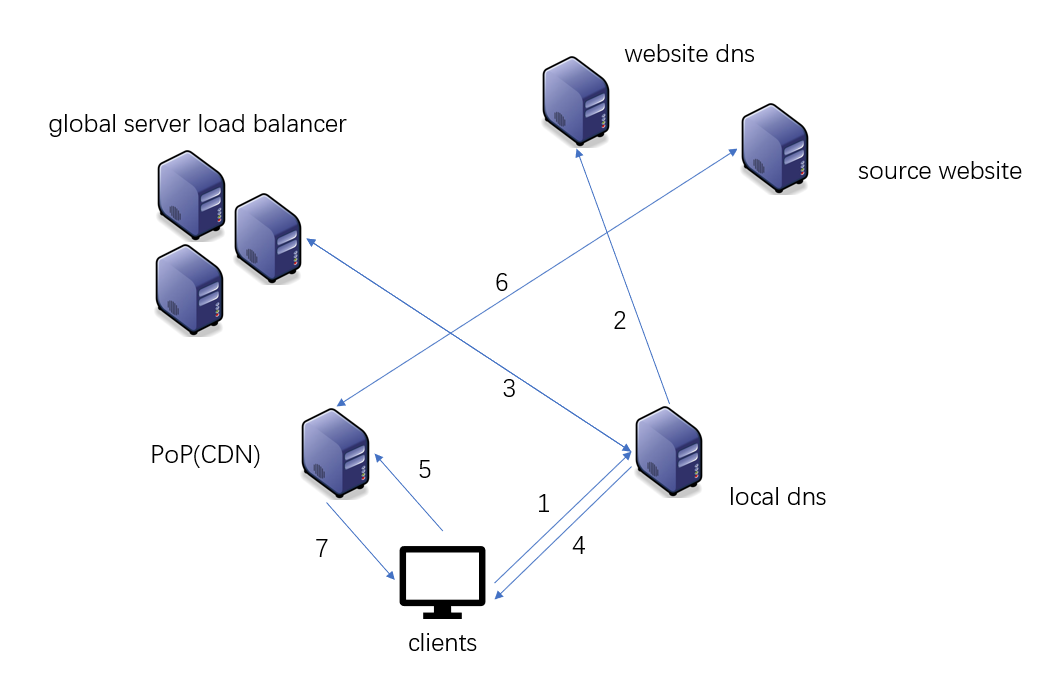
\includegraphics[width=0.5\textwidth]{CDN_new.png}
    \caption{The basic working procedure of CDN}
    \label{fig}
\end{figure}

\begin{figure}[h]
    \centering
    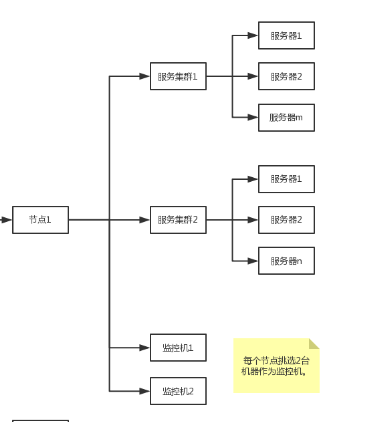
\includegraphics[width=0.5\textwidth]{cache_group.png}
    \caption{The figure}
    \label{fig: the structure of PoP}
\end{figure}

A content delivery network or content distribution network (CDN) (figure 1) is a geographically distributed network of cache servers. CDN helps content provider deliver web pages and other multi-media content to the clients, based on the locations of the clients and cache servers nearby the clients. The basic working procedure is as follows. Step 1:client send a request to local dns. Step 2: the DNS finds the CNAME and redirects the request to the gslb (global sever load balance). Step 3: the local DNS server sends request to the glsb and glsb returns the ip address of CDN servers based on the scheduling policy. Step 4: the local DNS return the ip address to the clients. Step 5: clients make a request to fetch content from the selected PoP. Step 6: the cache server groups will pull the content from source website if the content doesn't exsist locally. Step 7: content is sent to the clients.

A CDN cache server group is the basic resource scheduling unit for CDN. A CDN cache group is a load balanced cluster that consists of interconnected cache servers. A typical implementation consists of HAproxy and squid servers. The requests from clients are distributed by HAproxy to cache servers. HAproxy use be set to use different algorithms algorithms to maximize the utilization of every server. Round-robin algorithm distributes the load equally to each server. In heterogeneous cluster,  weighted round-robin algorithm is used. A weight was assigned to the server based on its processing capabilities. A heterogeneous structure of a cluster adds complexity to the feature engineering.

As CDN providers don't have direct QoS measurement from the clients (the logs from video players, web browser that can show the QoE), so they use the indirect measurement \dabiaolv which is calculated from log of the HA proxy of CDN cache groups with a delay about three minutes. 

The number of metrics we collected from the cache servers of cache group are different due to the different configuration, from 64 to 134. The features we have constructed are listed in table. There are about 312 features. They include cpu utilization, network utilization, disk utilization, memory utilization and so on.

\begin{table}[]
\centering
\begin{tabular}{|c|}
\hline  
feature list\\
\hline  
group 1\\
\hline  
cpu1.usage\\
cpu2.usage\\
...  \\
mem\_cached\\
mem\_buffers\_cache\_free\\
memory.swap\\ 
disk.used.sda1\\
disk.used.sda2\\
...\\
channeltraffic\_in\\
channeltraffic\_in\\
ioutil\_util\_sda\\
ioutil\_util\_sdb\\
ioutil\_util\_sdc\\
ioutil\_util\_sdd\\
...\\
iowait.wait\\
hitratio.port8101\\
hitratio.port8102\\
...\\
\hline  
group 2\\
\hline 
aggregate.cpu\\
aggregate.diskused\\
aggregated.ioutil\\
aggregate.CPU.max\\
....\\
\hline  
group 3\\
\hline 
aggregate.all\_machine.cpu\\
aggregate.all\_machine.diskused\\
aggregated.all\_machine.ioutil\\
aggregate.all\_machine.CPU.max\\
\hline
\end{tabular}
\caption{list of candidate input features from one cache server. We organize the features into groups. The first group is the raw data we directly collected from the caching servers. The second group are the features we construct based on statistics of the metrics of a single cache server. The third group are the features we construct based on the statistics of the metrics of the whole cache server groups}
\label{my-label}
\end{table}

\section{Problem Formulation and Models}
We argue that performance evaluation as a sequence learning problem. Since we are able to collect the caching servers performance metrics and network metrics at a certain time interval, we can use a sequence models to describe relationship between metrics collected from  cache groups and \dabiaolv

There are three categories of sequence learning problem, which are many to one, many to one and many one. Our goal is to model the relationship between a sequence collected metrics and \dabiaolv within a certain period of time, which is many to one. In general, we can use the following formulation to describe the prediction process.

Giving a sequence of vectors, $\{x_n\}=\{x_{\alpha} \in R^{d}|\alpha \in N\}, $ , where $d$ is the number of the features, we use $\{x_n\}$ to represent the sequence and $x_t$ to describe a data point at time t with $d$ dimensions.

Given another target sequence, $\{y_n\}=\{y_{\alpha} \in R|\alpha \in N\}$, our goal is to find the relation between$\{x_n\}$ and $\{y_n\}$, which is 
$$y_t=f(x_{t},x_{t-1},...,x_{t-n+1})$$
where $n$ is the window size and $f$ is the mapping we want to learn from the data.

Many models can be used to approximate $f$ in sequence modeling. The most naive way is to use simple heuristics, which is use exponential moving average to linearly map each metrics to a score in a certain time interval. The paremeters are depending on the experience of the operators. This methods are impractical: the model can hardly generalize well and requires tedious repetitive tuning.

\subsection{linear models for sequence learning}

There are conventional approaches which use data to learn: use the multiple linear regression model(MLR). The MLR method builds a model of a sequence that is composed of a linear part and a random noise part. The linear part models the linear relationship between the dependent variables and independent variables, the random noise reflects the unpredictable randomness. Formally, the model for multiple linear regression, given n observations, is 
    $$y_t = c+\sum_{i=t-n+1}^{t}(\beta_i ∗ x_{t_i})+\epsilon_t$$

Furthermore, the linear part incorporates historical values of the sequence. Here, y denotes the target we want to model, c denotes the constant parameter of the linear decomposition, β denotes the parameters to be computed and epsilon reflects the random noise part. The best-fitting line for the observed data is calculated by the least square method.


Linear models are easy to implement and have good interpretation and thus are widely used in many real work. However, linear models are shown not sufficient to describe some nonlinear behaviors of the complex network systems. In many cases, neural networks tend to outperform linear models [A comparison of artificial neural network and time series models for forecasting commodity prices]. In our experiments, we observe a non-linear relationship between the metrics and \dabiaolv.

Deep learning (DL) is a branch of machine learning based on a set of algorithms that attempts to model high-level abstractions in data by using artificial neural network (ANN) architectures composed of multiple non-linear transformations. They have a lot of successful applications in sequence modeling. Compared to other machine learning techniques, it can detect complex relationships among features, can extract hierarchical level of features from raw data. So it can produce more accurate result and build a model more accurate with less time. They are advantageous for modeling intricate systems because neural networks do not require the user to predefine the feature interactions in the model, which assumes relationships within the data. Instead, the neural network searches for patterns and interactions between features to automatically generate a best fit model.

One of the more popular kind of deep neural networks is the Recurrent Neural Network (RNN). RNNs are a class of neural networks that depend on the sequential nature of their input. Such inputs could be text, speech, time series, and anything else in which the occurrence of an element in the sequence is dependent on the elements that appeared before it.

\subsection{non-linear for sequence learning}
Sequence prediction often involves forecasting the next value in a real valued sequence or outputting a class label for an input sequence.

\subsubsection{Basic feed forward neural network}
\begin{figure}[h]
    \centering
    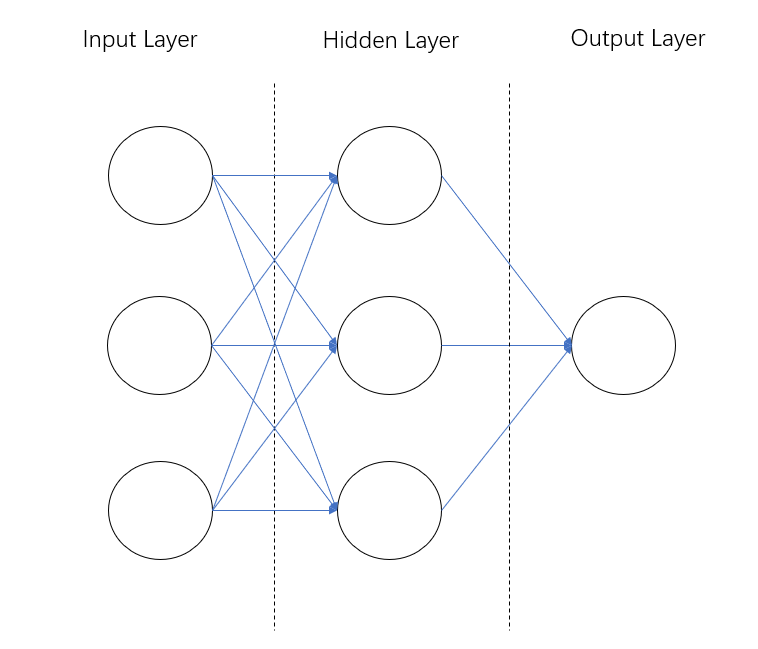
\includegraphics[width=0.5\textwidth]{mlp.png}
    \caption{MLP structure}
    \label{fig:RNN}
\end{figure}

A generic three layered neural network is illustrated in Figure 2. In this study, the input matrix $I \in R^{Mx(NxT+1)}$  where M is the number of training examples and $NxT+1$ is the number of features (metrics that collected from the cache servers) concatenating the bias term. The input matrix is then multiplied by the model parameters matrix $W_1$ to produce the hidden state matrix $h$. The Output of the first layer is transformed by an activation function. We can add more layers to the network. interacts with the second parameters matrix $\Theta^2$ to calculate the output $O$. The size and number of hidden layers can be varied to model systems of varying complexity. The whole process can be imagined as the information propagating forward. The forward propagation is formalized as follows:

\begin{equation}
    \begin{split}
    & \mathbf h_1 = \text{sigmoid}(\mathbf W_1 * \mathbf I) \\
    & \mathbf h_t = \text{sigmoid}(\mathbf W_{t-1} * \mathbf h_{t-1}) \\
    & \mathbf O=\text{sigmoid}(\mathbf W * \mathbf h_{lastlayer}) \\
    \end{split}
\end{equation}

where sigmoid is the activation function:
\begin{equation}
    \begin{split}
    & \text{sigmoid}(x)=\frac{1}{1+e^{-x}}
    \end{split}
\end{equation}

the loss function $J$ use mean square error:
    $J$

The process of training any neural network model can be broken down into four steps: (1) Randomly initialize the model parameters, (2) forward propagation algorithm,(3) Compute the cost function $J$, (4) back propagate using the chain rule  (5) using the gradients calculated, adjust weights to minimize the cost function $J$.

One major assumption for NNs is the independence of samples. For sequence learning problem, however, this assumption doesn't hold true, for the samples of our problem have a temporal relationship: the status of system of the next timestep not only depends on the status in the current timestep but also on the previous timesteps of indefinite length. One solution is to using a sliding window to capture the sequential relationship between the samples. The performance of this method depends on the window size, which isn't pratical for the dependencies length which isn't a fixed value. RNN eliminates the need to find the size of the window\cite{HermansTrainingNetworks}. 

\subsubsection{RNN}
The promise of recurrent neural networks is that the temporal dependence and contextual
information in the input data can be learned\cite{Bengio1994LearningDifficult} \cite{ChoLearningTranslation}. 

RNNs \ref{fig:RNN} process the input sequence one element at a time and maintain a hidden
state vector which acts as a memory for past information. They learn to selectively retain relevant information allowing them to capture dependencies across several time steps. This allows them to utilize both current input and past information while making future predictions. All this is learned by the model automatically without much knowledge of the cycles or time dependencies in data. RNNs obviate the need for a fixed size time window and can also handle variable length sequences. Moreover, the number of states that can be represented by an NN is exponential in the number of nodes.

 
\begin{figure}[h]
    \centering
    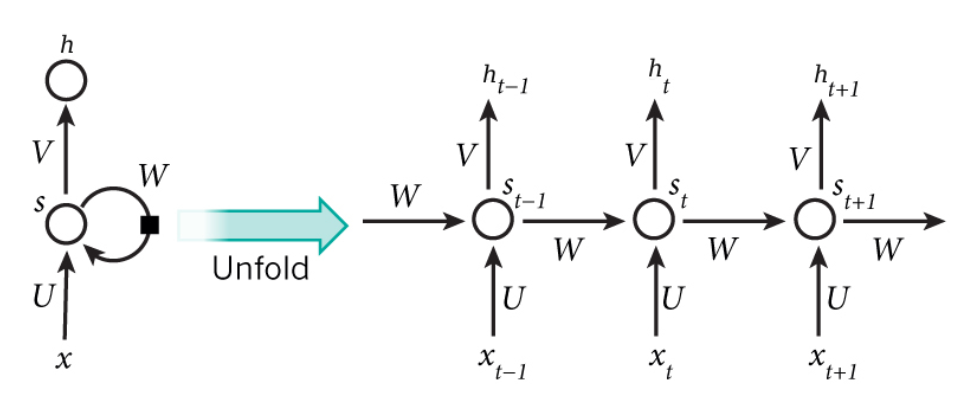
\includegraphics[width=0.5\textwidth]{RNN.png}
    \caption{The left shows the backloop structure of RNN and right shows that RNN can be thought as infinite deep layers neural network unfolded along the dimension of time}
    \label{fig:RNN can be thought as infinite deep layers neural network along the dimensions of time}
\end{figure}


RNNs maintain a hidden vector $\mathbf h$, which is updated at time step $t$ as follows:

\begin{equation}
	\mathbf h_t = \tanh(\mathbf W * \mathbf h_{t-1} + \mathbf I * \x_t)
\end{equation}

where $\tanh$ is the hyperbolic tangent function, $\mathbf W$ is the recurrent weight matrix and $U$ is a input wight matrix. The hidden state $\mathbf h$ is then used to make a prediction

\begin{equation}
	\mathbf y_t = f(\mathbf W * \mathbf h_{t-1})
\end{equation}

where $f$ can be fully connected layer that linearly maps the hidden state to an output. By using $\mathbf h$ as the input to another RNN, we can stack RNNs, creating deeper architectures 

\begin{equation}
	\mathbf h_t^{l} = \sigma(\mathbf W * \mathbf h_{t-1}^{l} + \mathbf I * \mathbf h_t^{l-1}).
\end{equation}

The training of RNN use back-propagation through time (BPTT). Training vanilla RNNs is known to be particularly difficult, with vanishing and exploding gradients being one possible explanation \cite{pascanu2012difficulty}. The LSTM introduced in the next section address this problems

\subsubsection{LSTM}
LSTM, introduced in \cite{Hochreiter1997LongMemory}, addresses the problem of vanishing gradients by introducing a memory cell. \cite{MalhotraLongSeries} applied in time series. The inner working of LSTM are listed follows:

\begin{equation}
	\begin{split}
		& \mathbf g_u = \sigma(\mathbf W_u * \mathbf h_{t-1} + \mathbf I_u * \x_t) \\
		& \mathbf g_f = \sigma(\mathbf W_f * \mathbf h_{t-1} + \mathbf I_f * \x_t) \\
		& \mathbf g_o = \sigma(\mathbf W_o * \mathbf h_{t-1} + \mathbf I_o * \x_t) \\
		& \mathbf g_c = \tanh(\mathbf W_c * \mathbf h_{t-1} + \mathbf I_c * \x_t) \\
		& \mathbf m_t = \mathbf g_f \odot \mathbf +  \mathbf g^u \odot \mathbf g^c \\
		& \mathbf h_t = \tanh(\mathbf g_o \odot \mathbf m_{t-1}) 
	\end{split}
\end{equation}

here $\sigma$ is the logistic sigmoid function, $\mathbf W_u, \mathbf W_f, \mathbf W_o, \mathbf W_c$ are recurrent weight matrices and $\mathbf I_u, \mathbf I_f, \mathbf I_o, \mathbf I_c$ are projection matrices.


\subsubsection{LSTM auto-encoder}
\cite{ChoLearningTranslation}
\begin{figure}[h]
    \centering
    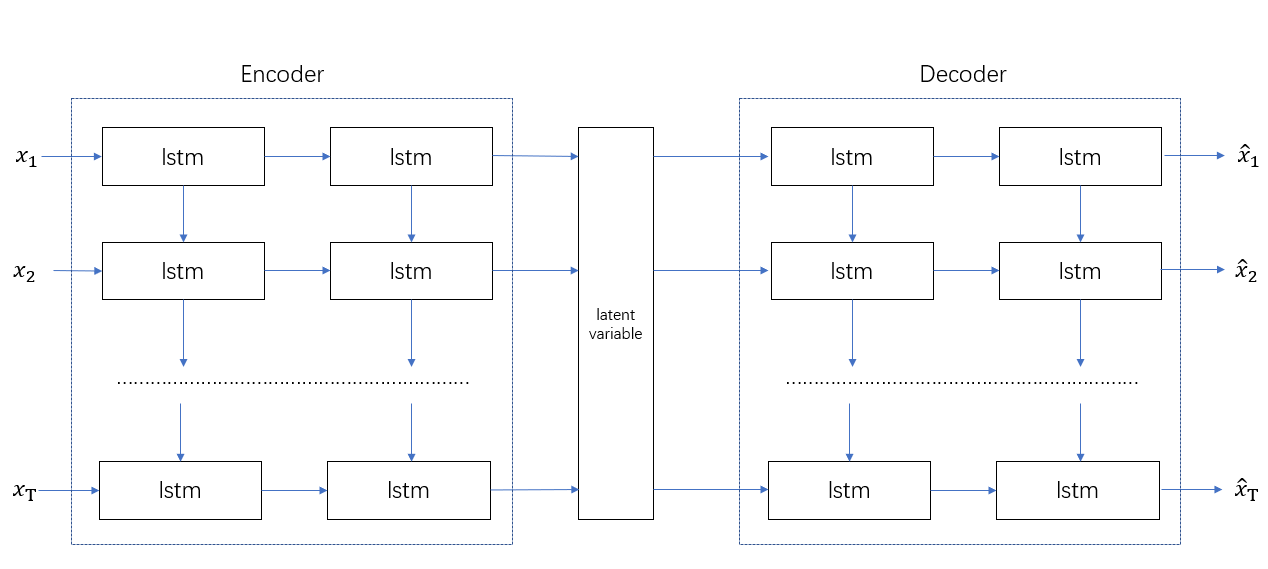
\includegraphics[width=0.5\textwidth]{auto_encoder.png}
    \caption{LSTM Auto-encoder Model}
    \label{fig:RNN_encoder-decoder}
\end{figure}

An autoencoder contains: an encoding function, a decoding function, and a distance function between the amount of information loss between the compressed representation of your data and the decompressed representation (i.e. a "loss" function). The encoder and decoder will be chosen to be deep layered lstm network. So the parameters of the encoding/decoding functions can be optimize to minimize the reconstruction loss, using Stochastic Gradient Descent.  


\section{Methods}
\subsection{Feature Engineering}
The feature engineering is the process after data-cleansing, in which we fill the missing data and reformat it. The propose of this stage is two-fold:
(1) to find a unified equal-length vector representation of all of the cache groups. 
The metrics collected are in the granularity of caching servers which have different dimensionality. As showed in graph. To make things more complex, a cache group may have different number caching servers. As we only care about. 
(2) reduce the dimensionality, for it is very time-consuming to train the models when the number of dimensionality is too high.

Our feature engineering has three steps: 1. data prepossessing which converts raw data into high-dimensional vectors. 2. feature correlation that characterize the linear relationship between every pair of features. 3. cluster analysis that selects the set of features.

\begin{figure}[h]
    \centering
    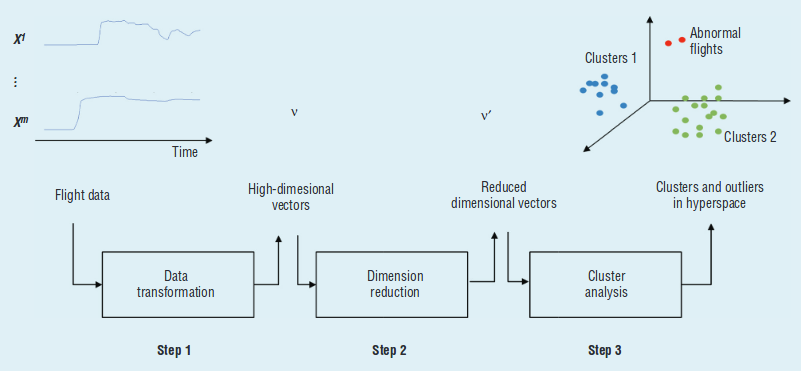
\includegraphics[width=0.5\textwidth]{feature_engineering.png}
    \caption{three steps of feature enginnering}
    \label{fig:Correlation_matrix}
\end{figure}

As there are hundreds of features, there are many overlaps among the variables. We use correlation in statistics to group highly correlated variables together and create composite features that can represent each group of variables.

Correlation is an analysis of two or more observed or random variables to determine a dependence between the variables. This dependence can be classified as the probability that changes in one variable affect the behaviour of the second variable. The Pearson’s correlation defines this dependence in the interval [−1.0, 1.0]. Pearson’s correlation for two given random variables X and Y is computed by dividing the covariance of both variables with the product of their standard deviations.

Generally, cases of high correlation compute to a value close to 1.0, high anticorrelation is associated with a value close to -1.0 and no correlation is assumed. if the value is around 0.0, the variables appear to be independent. 

The correlation matrix we calculate is pictured in figure \ref{fig:Correlation_matrix}. The white color denotes the correlation of 1.0 and the black denotes -1.0. The red denotes that there is no linear relationship at all. As we can see from the picture that there are overlaps among the features.

\begin{figure}[h]
    \centering
    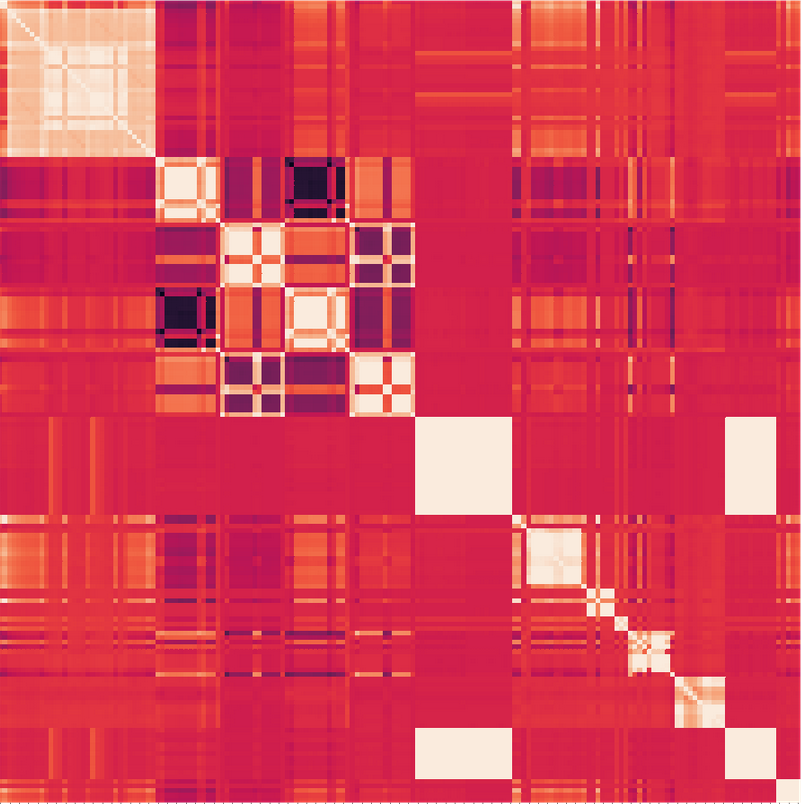
\includegraphics[width=0.5\textwidth]{Correlation_Matrix.png}
    \caption{Correlation Matrix of the feature set}
    \label{fig:Correlation_matrix}
\end{figure}

After we calculate the correlation matrix for all the features. We use DBSCAN to cluster these features to eliminate duplicated ones.

\begin{algorithm}[t]
\caption{Feature Aggregation and Selection} 
\begin{algorithmic}[1]
\Require  
    All features list: $F$;
    Neighborhood parameter $\epsilon$; 
\Ensure  
    Selected features list: $F_S$;  
\State Initialize the set of core object:  $\Omega$=$\emptyset$;
\For{$i \;in\; F$}
    \State Confirm the $\epsilon$-neighborhood\; N(i,$\epsilon$);
    \If {$|N(i,\epsilon)|$\textgreater 1} % If 语句,需要和EndIf对应
            \State Add i to the core object set: $\Omega$;
          \Else
            \State Add i to the selected features list: $F_S$;
        \EndIf
\EndFor
\State Initialize the number of clusters:  $k$=0;
\State Initialize the set of features:  $\Gamma$= $\Omega$;
\While{$\Omega\neq\emptyset$}
\State Check the set of unvisited features: $\psi$= $\Gamma$;
    \State Random select an core object $o$ $\in$ $\Omega$,initilaize the queue $Q$=$\langle o \rangle$;
\State $\Gamma$=$\Gamma \verb|\|\left\{o\right\}$;
\While{$Q\neq\emptyset$}
    \State Fetch an element from Q: $q$;
    \State $\Delta=N(q,\epsilon)\bigcap\Gamma$;
    \State Add the elements in $\Delta$ to Q;
    \State  $\Gamma= \Gamma\verb|\|\Delta$;
\EndWhile
\State $k=k+1$;
\State Generate the cluster C$_k$=$\psi\verb|\|\Gamma$;
\State $\Omega=\Omega\verb|\|C_k$;
\EndWhile
\For{i=1,2...k}
    \State Fetch an element in $C_k$ out to the selected features list $F_s$
\EndFor
\State \Return $F_s$
\end{algorithmic}
\end{algorithm}


\subsection{Prediction Model Design}

In this section, we introduce how the architecture we use to predict \dabiaolv of CDN cache group using the data output from the feature engineering stage. 

Prior to fitting the data prediction model, we first conduct a pre-training step to fit an encoder that can extract useful and representative embeddings froma  time  series.  The  goals  are  to  ensure  that  (i)  the  learned embedding  provides  useful  features  for  prediction  and  (ii) unusual input can be captured in the embedded space, which will get further propagated to the prediction network in the next step.

\begin{figure*}[h]
    \centering
    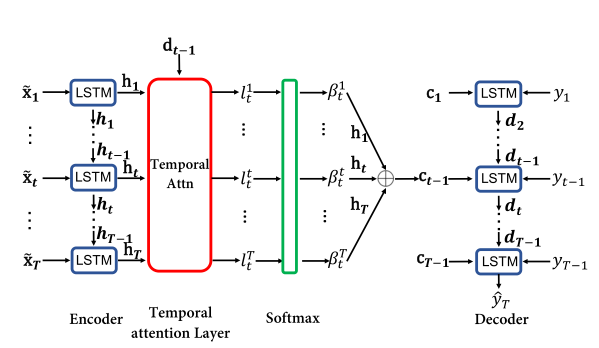
\includegraphics[width=0.8\textwidth]{our_models.png}
    \caption{lstm auto-encoder with a deep feadfoward network}
    \label{fig:our_models}
\end{figure*}

As illustrated in figure \ref{fig:our_models}. Given a multi-variate time series of data, the encoder reads the vectors as input and transform them as latent variables. The latent variables are  

\section{Evaluation}
\subsection{Experimental Settings and Dataset}
Our implementation uses the Google opensource deep learning library, Tensorflow, version 1.2.0. We ran our experiments on a physical machine running an Ubuntu 16.04 operation system, intel i7-6700HQ, 16 GB memory, and GPU gtx1060.

To test the performance, we select two cache groups with average request above. The first cache servers groups have 13 cache servers while the other have 10 cache servers. The  metrics are raw data collected from the cache servers, including cpu utilization, network utilization, disk utilization, memory utilization of two cache groups servers. The frequency of the metrics and  \dabiaolv are both minute-by-minute. This data covers the period from November 26, 2016 to January 20 22, 2018, 105 days in total.

In the experiments, 10-fold cross validation is used to evaluate the accuracy of predictions. This divides the entire data set into 10 equal parts.  Prediction is repeated 10 times, each time keeping one of the 10 parts as test data and the other 9 parts as training data to build the prediction model. Finally, test results on all the 10 parts are accumulated together to calculate the average prediction accuracy.

In the pre-training procedure We use minibatch stochcasti  gradient descent (SGD) together with the Adam optimizer to train model. The size of the minibatch is 128. The weights can be learned by standard lstm learning algorithm propagation throught with mean squared error as the objective function.

In the training procesure we use a 4 layer feed-foward neural network. We use the batch gradient descent training algorithm to train the neural network.

\subsection{Baseline}
We compare our model with other baseline model which are listed follow:
\begin{enumerate}
  \item multiple linear regression model
  \item basic three layer feed-foward neural network
  \item vanilla LSTM model
  \item LSTM encoder-decoder with feed-foward neural network
\end{enumerate}

We use three different evaluation metrics to compare our models and methods. Among them, root mean squared error (RMSE) and mean absolute error (MAE) are two scale-dependent measures, and mean absolute percentage error (MAPE) is a scale-dependent measure. Specifically, assuming $y^'$ is the target at time t and $y$ is the predicted value at time t. 


\begin{equation}
    RMSE(y^{'},y)=\sqrt{\frac{1}{n}\times{\sum_{n=1}^N(y^{'}{_t}-y_t})^2}
\end{equation}

\begin{equation}
	 MAE(y^{'},y)=\frac{1}{N}\times\left| y^{'}{_t}-y_t \right|
\end{equation}

\begin{equation}
	 MAPE(y^{'},y)=\frac{1}{N}\times\left| \frac{y^{'}{_t}-y_t}{y^'_t} \right|
\end{equation}

\begin{table*}[]
\centering
\caption{Performance Comparison}
\label{my-label}
\begin{tabular}{|l|l|l|l|}
\hline
Models & MAE & MAPE & RMSE\\
\hline
multiple linear regressionmodel & 10.0 & 9.9  & 8.8 \\
\hline
feed-foward neural network with sliding windows & 10.0 & 9.9  & 8.8 \\
\hline
RNN & 0.21 & 0.12  & 0.141 \\
\hline
LSTM encoder-decoder with feed-foward neural network& 10.0 & 9.9  & 8.8 \\
\hline  
\end{tabular}
\end{table*}

\begin{figure*}[h]
    \centering
    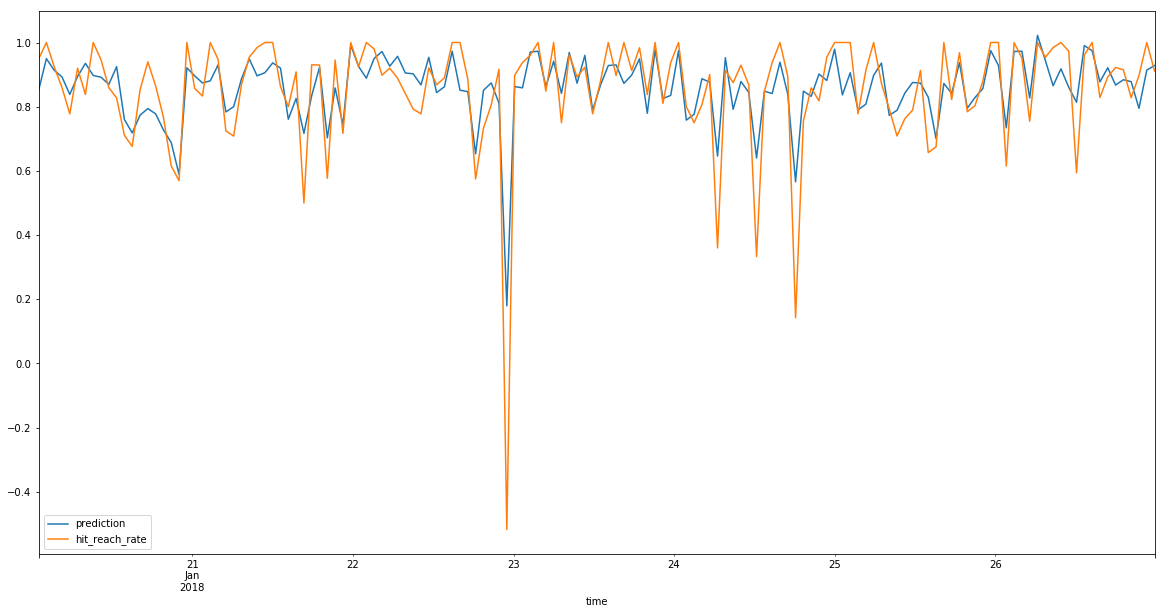
\includegraphics[width=0.8\textwidth]{result.png}
    \caption{Prediction Results of LSTM auto-encoded with feed-forward neural network}
    \label{fig:Prediction Results}
\end{figure*}

\begin{figure*}[h]
    \centering
    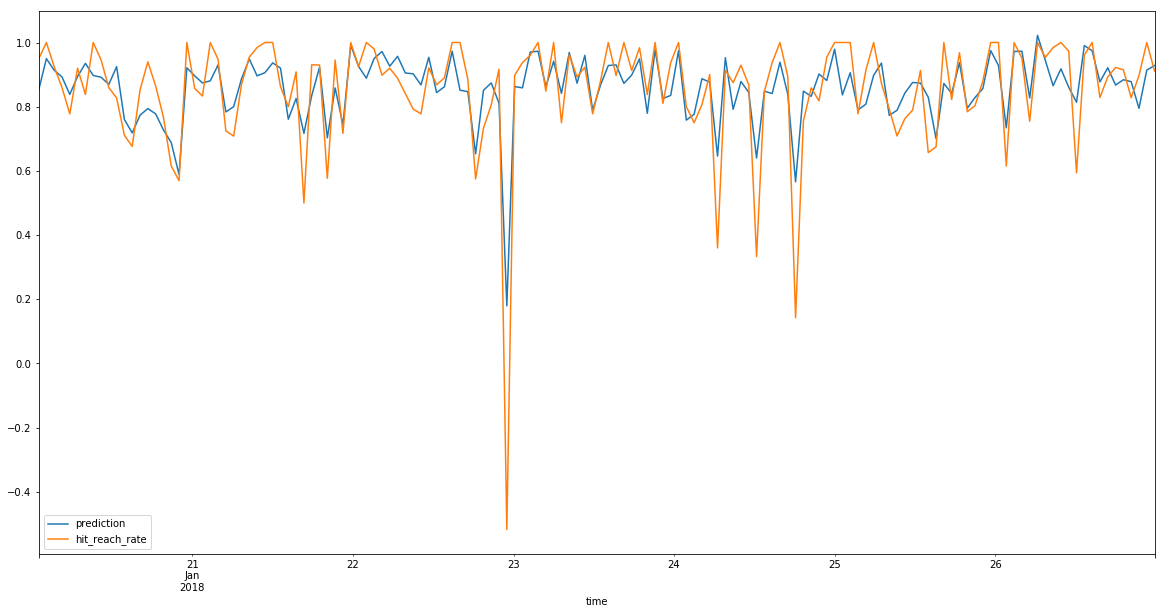
\includegraphics[width=0.8\textwidth]{result.png}
    \caption{errors comparaison of different models}
    \label{fig:Prediction Results}
\end{figure*}

error over diffenrent models
 
\section{Related Work}
In recent year, deep learning has gained success in different fields, including image recognization, speech recognization, natural language understanding\cite{Lecun2015}. RNN\cite{Schmidhuber1989} outperform the traditional feed-forward neural network in modeling sequence data because its structure can characterize the temporal structure of input data by introducing hidden state. Training RNN is hard because of vanishing gradients problem; LSTM address these issues by introducing LSTM cell\cite{Hochreiter1997LongMemory}. LSTM has been widely proven successful in sequence modeling. In \cite{Qin}, a attention-based lstm outperforms traditional methods like ARIMA. In \cite{Zhu2017DeepUber}, a robust model was used to predict number of trips and do anomaly detection for Uber. 

When evaluating the complex system, the evaluation method can fall into two catagory: model-driven method, data-driven method. In model-driven method, the mathematical model characterizing the inner components of a system has to be explained explicitly. In \cite{Tang2017RethinkingDemands}, a model-driven method is used to solve optimal cache-deployment problem. However, in data-driven method, the data characterizing the behaviour of system instead of the analytical model is necessary. In \cite{Jiang2017Pytheas:Exploration-Exploitation}, CDN selection decisions of QoE optimization decision is based on the past experience of decisions and decisions outcome. In \cite{Mao2017NeuralPensieve}, a ABR decision framework using deep reinforcement learning treats network as a black box. In \cite{Zhao2017LearningNetworks}, a convolutional bi-directional LSTM network is used to predict the machine health by sensor data. in \cite{Yadwadkar2017SelectingClouds}, the VM selection mechanism allows users to balance performance gains with cost reductions. From the characteristics of the above methods, the data driven method, which takes the gathered data as basis and is independent of the object’s prior knowledge, is a more useful approach for performance evaluation, fault detection and reliability evaluation.

There are extensive research regarding CDN, for a large portion of internet traffic was boosted by service provided by CDN. There are three category: (1) long-term network planning, including optimized CDN design that relates to PoP selection and cache deployment\cite{Krishnan2000}\cite{Hasan2014}\cite{Tang2017RethinkingDemands}, and (2) short-term, run-time cache management, including content replacement and prefetching strategies in the CDN network\cite{Borst2010}\cite{Leconte2016}\cite{Applegate2016}. (3) CDN selection to optimize QoE for the client\cite{Jiang2017Pytheas:Exploration-Exploitation}\cite{JiangCFA:Optimization}. Our research falls in the second categories.

\section{Conclusion and Future Work}

In this paper we present a data-driven approach to evaluate the performance of cache server groups. The lstm auto-encoder can capture the long-term temporal information in the sequences. This paper shows that it is feasible to apply state-of-the-art deep learning techniques to model networked systems that provides estimation for its performance. The empirical studies shows that ours has outperformed the conventional methods.

%As there are hundreds cache group in China. Although our method can be used to train on all kinds of cache group of different architecture, the model for one specific cache group, a unified models for all kinds of cache groups is required. As qualified rate is an indirect measurement of QoS of clients, collecting data from clients ends will provide useful insights. We also want to develop the online training methods for our models because we observe that the relationship change over time.

\section{Acknowledgment}
The work of this paper is supported by National Natural Science Foundation of China under Grant No.61728202-Research on Internet of Things Big Data Transmission and Processing Architecture based on Cloud-Fog Hybrid Computing Model & Grant No. 61572137-Multiple Clouds based CDN as a Service Key Technology Research, and Shanghai 2016 Innovation Action Project under Grant 16DZ1100200-Data-trade-supporting Big Data Testbed.


\section*{References}
\bibliographystyle{unsrt}
\bibliography{mendeley}
\end{document}